\chapter{Definition of Chow ring}
\begin{center}
	{\huge Speaker: Andrea Gallese}
\end{center}
\bigskip

\noindent
The main reference for this chapter is \cite{eisenbud20163264}.

\section{Algebrizing intersection}
Think back to our roots: algebraic geometry is the study of solutions to systems of polynomial equations, which we can think of as intersecting some geometric objects. It seems reasonable then that we ought to study carefully what it means for varieties to intersect. 

One way we may approach this question can we make intersection into an algebraic operation? The answer is yes and the algebraic objects which come out from this idea are the Chow rings.

\bigskip

\noindent
In this chapter we take $k$ to be an alegbraically closed field. All schemes will be smooth and of finite type\footnote{note that this implies noetherian} over $k$.

\subsection{Chow group}
\begin{definition}[]
Let $X$ be a scheme as above. We define its \textbf{algebraic cycles} to be
\[Z(X)=\Z\spa{\text{integral closed subschemes of $X$}}=\bigoplus_{k}Z_k(X).\]
where $Z_k(X)$ is the same thing for subschemes of dimension $k$.
\end{definition}

\begin{remark}
$Z(X)=Z(X^{red})$.
\end{remark}

\begin{remark}
We may also grade $Z(X)$ with respect to codimension instead of dimension, which we will do eventually.
\end{remark}


\begin{definition}
Given $Y\subseteq X$ closed subscheme with irreducible components $Y_1,\cdots, Y_r$, we define the \textbf{algebraic cycle associated to $Y$} to be
\[\ps{Y}=\sum_{i=1}^r \ell_i[Y_i]\]
where\footnote{length of the module over itself. In particular, if $\Oc_{Y,y_i}$ is reduced then $\ell_i=1$.} $\ell_i=\length(\Oc_{Y,y_i})$ for $y_i\in Y_i$ the generic point.
\end{definition}

\begin{example}
Consider $V(xy)\subseteq \A^2$. The irreducible components are $V(x)$ and $V(y)$ with generic points $(x)$ and $(y)$ respectively. Note that $\pa{\frac{k[x,y]}{(x)}}_{(x)}=k(y)$, so it is reduced and the length is 1, same idea for the other irreducible component.
\medskip

Consider now $V(x^2)\subseteq \A^2$. The only irreducible component is $V(x)$ with generic point $(x)$ but now $\pa{\frac{k[x,y]}{(x^2)}}_{(x)}$ is not reduced because $x\neq 0$ and $x^2=0$. This is reflected in the fact that this ring has length 2, which can be seen by noting that
\[(0)\subsetneq (x)\subsetneq (1)\]
is a composition series. The fact that the length is 2 recovers the fact that we started with $V(x^2)$ instead of $V(x)$.
\end{example}

The group of cycles is way too large for any practical purpose, so we want to define when two cycles should be thought of as the same. We give the following definition in hope that it models ``continuous deformations" in some sense:

\begin{definition}[]
We define the subgroup $\Rat(X)$ of $Z(X)$ to be the one which is generated as follows
\[\Rat(X)=\ps{\ps{\Phi\cap (\cpa{t_0}\times X)}-\ps{\Phi\cap (\cpa{t_1}\times X)}}\]
where $Z$ varies among integral subvarieties of $X\times \Pj^1$ and $t_0,t_1$ are rational points of the projective line, i.e. $t_0,t_1\in \Pj^1(k)$.
\end{definition}

We can now define our main character

\begin{definition}[]
Let $X$ be a smooth scheme of finite type over $k$. We define its \textbf{Chow group} as the quotient
\[CH(X)=\frac{Z(X)}{\Rat(X)}.\]
If two cycles give the same element in $CH(X)$ we say that they are \textbf{rationally equivalent} and we may write this with $\sim$.
\end{definition}

\begin{remark}
The Chow group is graded by dimension and by codimension.
\end{remark}

\begin{example}
The cycles $[y=0]+[x=0]$ and $[xy=1]$ in $\A^2$ are rationally equivalent. Consider 
\[\Phi=V(xy-t)\subseteq \Pj^1\times \A^2\]
where $t$ is the coordinate\footnote{to be more precise, if the coordinates are $[s:t]$ we are taking $\Phi=V(sxy-t)$} of $\Pj^1$. Let $t_0=0$ and $t_1=1$, which are clearly rational points of $\Pj^1$, then we have
\[[y=0]+[x=0]=\ps{V(xy)}=\ps{\Phi\cap \cpa{0}\times \A^2}\]
and similarly for the other cycle. Thus $[y=0]+[x=0]\sim [xy=1]$.
\begin{figure}[!htb]
	\centering
	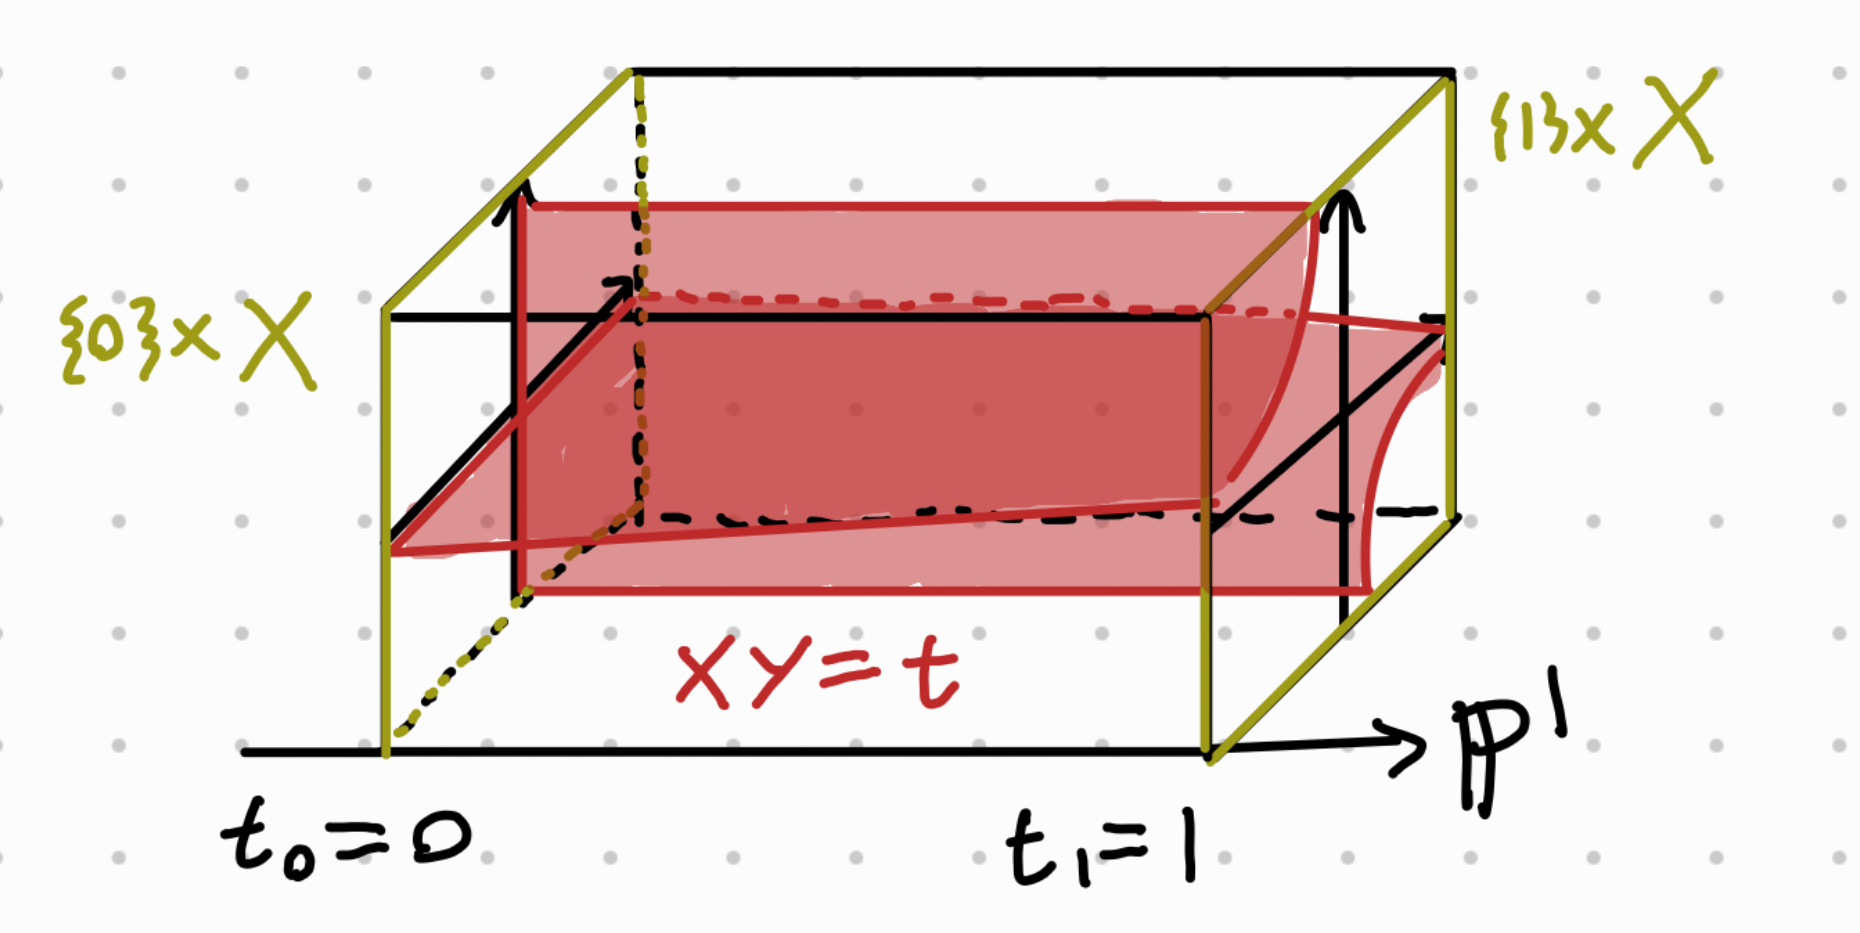
\includegraphics[width=9cm]{Images/rational-equivalence.png}
\end{figure}
\end{example}

\begin{remark}
It may be useful to think of rational equivalence as some type of homotopy equivalence. This would make the Chow ring something akin to the cohomology ring of the varieties. These analogies are beatiful and deep, but we shall not persue them further.
\end{remark}



\begin{example}
In $\A^2$ all points are rationally equivalent. To find the relation just multiply $\Pj^1$ with $\A^2$ and consider the line which connects the two points at different slices like in the picture
\begin{figure}[!htb]
	\centering
	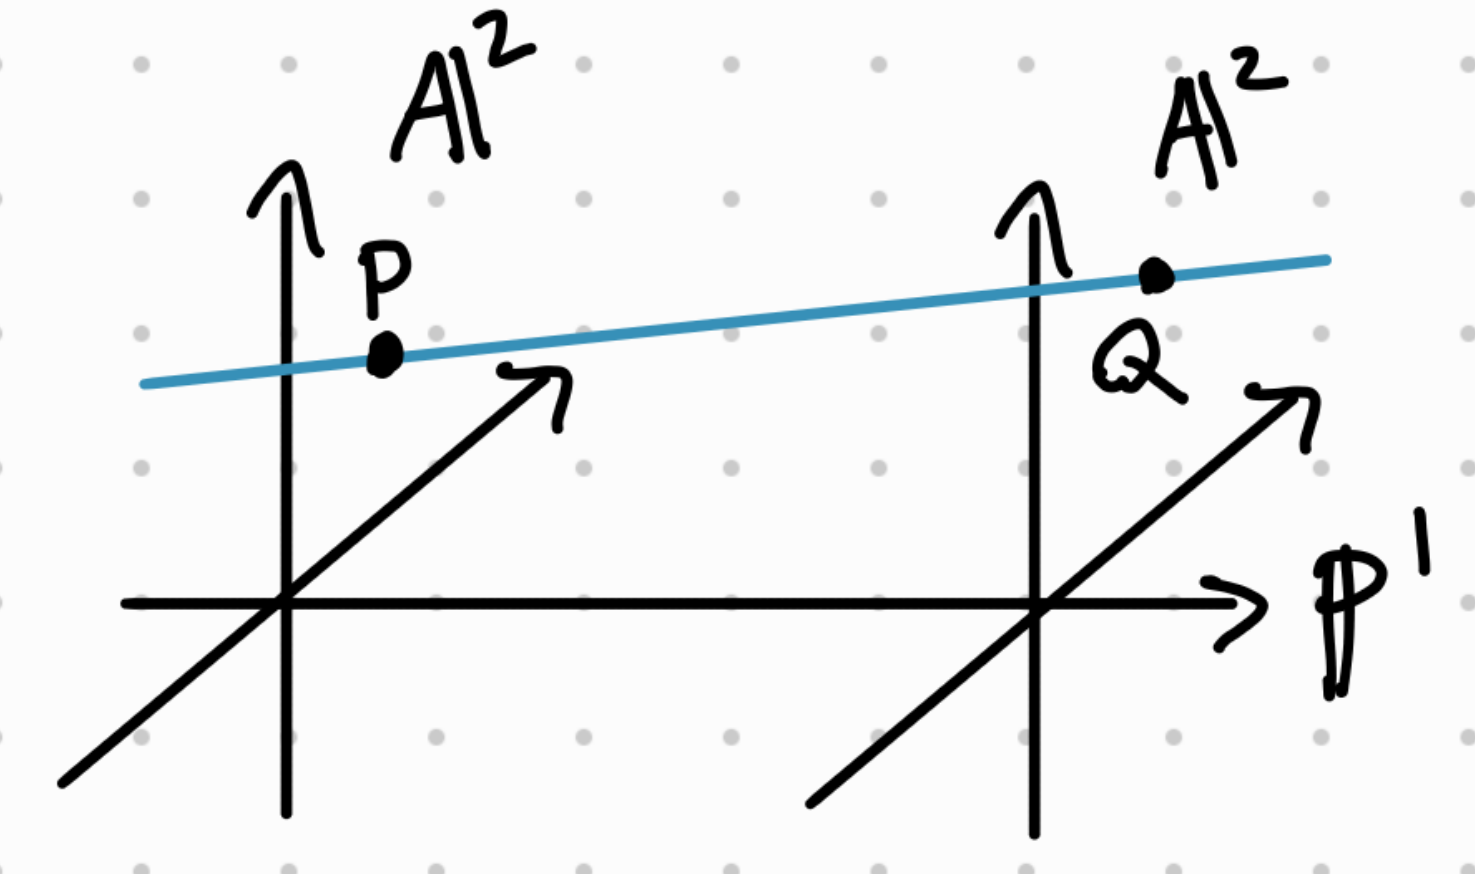
\includegraphics[width=6cm]{Images/points-in-A2-are-rationally-equivalent.png}
\end{figure}
\end{example}

\begin{example}
In $\A^2$, all lines passing through the origin are rationally equivalent.
Recall that $\GL_2$ acts on $\A^2$ and that $\GL_2\subseteq \A^4$. Moreover, the orbit of some line $L$ under the action of $\GL_2$ yiels all lines. This suggests a way to construct a rational equivalence between $[L]$ and $[gL]$ for $g\in \GL_2$.

The idea is to take the line $g(t)$ in $\A^4$ which connects $id\in \GL_2$ to $g\in \GL_2$ and then consider $\Phi$ to be the variety where each slice corresponds to $g(t)L$.
\end{example}


\subsection{Chow ring}
Now that we have our objects that we want to intersect, we want to count the ``number of intersections" somehow. 

If we think about this, we find a problem when trying to define what the intersection ought to be when tangencies are involved. For example, if we intersect a line with a circle we always get two intersection points except when the line is tangent to the circle, in which case the two intersection points \textit{collapse} to a single point. We want to count that as an intersection of multiplicity 2, not a single intersection.

\begin{figure}[!htb]
	\centering
	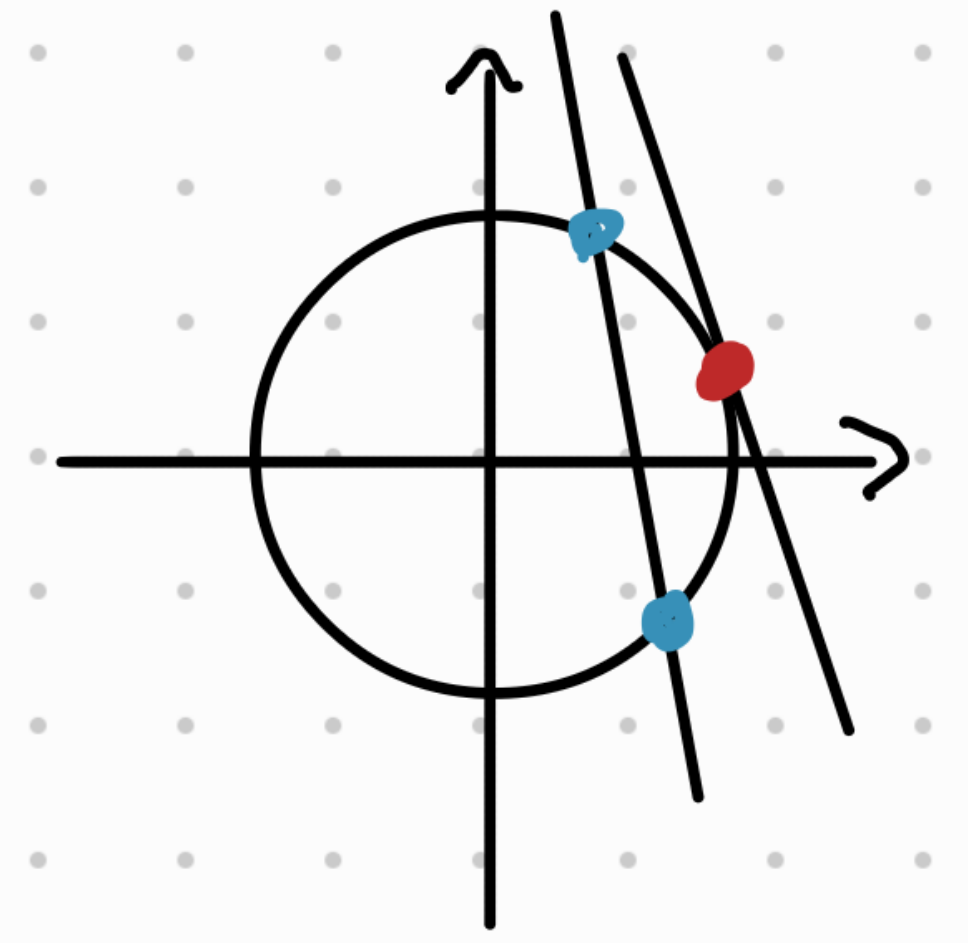
\includegraphics[width=4cm]{Images/tangent-moves-to-transverse.png}
\end{figure}

Let us define the ``well behaved" cases of intersection first:

\begin{definition}[]
Let $A,B$ be integral subvarieties of $X$. We say that $A$ and $B$ are \textbf{transverse} at $p\in A\cap B$ if $T_pA+T_pB=T_pX$, i.e. 
\[\codim T_p A+\codim T_p B=\codim(T_pA\cap T_p B).\]
We say that $A$ and $B$ are \textbf{generically transverse} if they are transverse at all generic points of the intersection.
\end{definition}

We now cite a lemma which tells us that we may reduce ``ill behaved" cases to ``well behaved" ones

\begin{lemma}[Moving lemma]
Let $X$ be a smooth quasi-projective variety, then the following holds:
\begin{itemize}
\item For all $\al,\beta\in CH(X)$ there exist $A,B\in Z(X)$ such that $\al=[A]$, $\beta=[B]$ and $A,B$ are generically transverse.
\item The class $[A\cap B]$ depends only on $[A]$ and $[B]$, not the representatives $A,B$.
\end{itemize}
\end{lemma}

With this lemma we can now put a product on $CH(X)$ which formalizes intersection, making it a ring.

\begin{theorem}
Let $X$ be smooth and quasi-projective, then there exists a unique product on $CH(X)$ such that for all $A,B$ subvarieties of $X$, if they are generically transverse then $[A]\cdot [B]=[A\cap B]$.

This makes $CH(X)$ into a graded (by codimension), associative, commutative and unital ring.
\end{theorem}

\begin{remark}
The identity of the Chow ring of $X$ is the \textbf{fundemental class}, i.e. $[X]$. This has degree (codimension) $0$ as we would expect. Intuitively, this corresponds to the simple fact that
\[A\subseteq X\implies A\cap X=A.\]
\end{remark}


\subsection{Non-triviality}

The first non-triviality result concerns codimention 0 cycles, that is, irreducible components of the ambient variety.
\begin{theorem}
If $X$ is irreducible and $\dim X=n$ then $CH_n(X)=CH^0(X)\cong \Z$ and it is generated by $[X]$.

If $X$ has irreducible components given by $X_1,\cdots, X_r$, then $[X_1],\cdots, [X_r]$ generate a free abelian subgroup of $CH(X)$ which is isomorphic to $\Z^r$.
\end{theorem}
\begin{proof}[Sketch]
If $\Phi\subseteq X\times \Pj^1$ gives some rational equivalence then $\Phi\subseteq X_i\times \Pj^1$ by irreducibility. So we may only consider the irreducible case.
If $\Phi\cap (\cpa{t_0}\times X)=X$ then $\Phi=X\times \Pj^1$, again by irreduciblity.
\end{proof}

\noindent
When considering codimension 1 we get back the theory of divisors as one would expect
\begin{proposition}
Suppose $X$ is irreducible of dimension $n$, then
\[CH_{n-1}(X)=CH^1(X)\cong \Pic(X)\]
and the correspondence is that the divisor $D=\sum n_i Y_i$ corresponds to $\sum n_i[Y_i]$.
\end{proposition}
\begin{proof}[Rough sketch]
The correspondence is clear at the level of $Z(X)$ and $\Div(X)$. What we need to see is that the two equivalence relations translate into each other.
If $f\in k(X)$ then we may take $\Phi=V(f(x)-t)$ to see that $[\cpa{f=0}]=[\cpa{f=\infty}]$, so $\mathrm{div}(f)$ does map to something in $\Rat(X)$.
To conclude we would need to show that $\Rat(X)$ is generated by the relations induced by principals divisors in this way.
\end{proof}


\section{Mayer-Vietoris and Excision}

Given the resemblance we noted before with cohomology rings, the following theorems seem rather natural (though we will not provide proofs):

\begin{theorem}[Mayer-Vietoris]
Let $X_1,X_2\subseteq X$ closed subvarieties, then we have an exact sequence
\[CH(X_1\cap X_2)\to CH(X_1)\oplus CH(X_2)\to CH(X_1\cup X_2)\to 0.\]
\end{theorem}


\begin{theorem}[Excision]
Let $Y\subseteq X$ be a closed subvariety, then we have an exact sequence
\[CH(Y)\to CH(X)\to CH(X\bs Y)\to 0\]
\end{theorem}




\subsection{Issue with Chow rings of affine space}

Having now defined Chow rings, we want to compute some of them explicitly. We might attempt this first with affine space, but we start to run into some issues


\begin{example}
If we think about the Chow ring of spaces like $\A^2$ we start to run into some problems. For example, consider $[C]^2$ for $C$ some circle. To compute this intersection we may move a little one copy of the circle as in the picture
\begin{figure}[!htb]
	\centering
	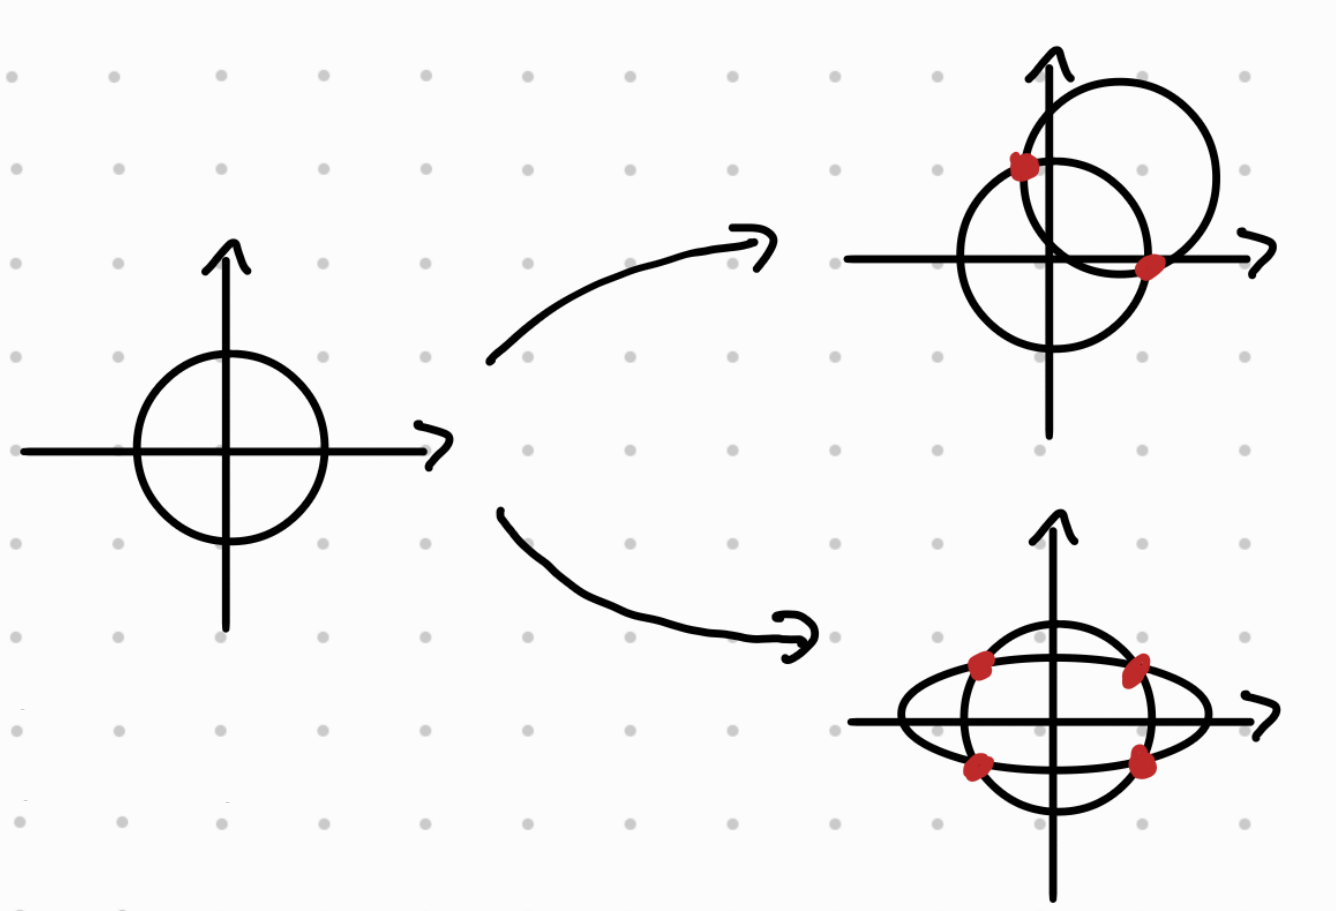
\includegraphics[width=8cm]{Images/circle-intersect-itself.png}
\end{figure}

The issue is that in the bottom case the four points of intersection are still in the affine plane, but in the top case they are at infinity, yielding some undesidered consequences which we will make more explicit in the next result.
\end{example}


\begin{proposition}
The Chow ring of affine space is $CH(\A^n)=\Z[\A^n]\cong \Z$, concentrated in degree 0.
\end{proposition}
\begin{proof}
Let $Y$ be any positive-codimension cycle and move it\footnote{translated copies of the same cycle are clearly rationally equivalent.} so that it does not pass through $0$.
We define\footnote{by $f(z/t)$ what we really mean is: if $t=x_1/x_0$ is the coordinate of $\Pj^1$, take $f$ and homogenize it with respect to $x_1$ to get $H_{x_1}(f)$. By the notation $f(z/t)$ we mean $(H_{x_1}(f)(x_0 z))/(x_1^{\deg f})$.}
\[\Phi=\cpa{(t,ty)\mid y\in Y,\ t\in \A^1}=V(\cpa{f(z/t)\mid f\in I(Y)})\subseteq \Pj^1\times \A^n.\]
Let us consider the slices of $\Phi$ at $t_0=1$ and $t_1=\infty$: 
\setlength{\leftmargini}{0cm}
\begin{itemize}
\item[$\boxed{t=1}$] The ideal is $I(Y)$ itself ($f(z/1)=f(z)$) and we get back $Y$.
\item[$\boxed{t=\infty}$] Since $Y$ does not go through $0$, there is some $f\in I(Y)$ such that $f(0)\neq 0$. If we take the slice at $\infty$ we get that $f(z/\infty)=f(0)\neq 0$ is in the ideal which defines $\Phi\cap \cpa{\infty}\times \A^n$, so the slice is $\emptyset$.
\end{itemize}
\setlength{\leftmargini}{0.5cm}
We have just shown that $\Phi$ defines an equivalence between $Y$ and $\emptyset$, meaning that all cycles in positive codimension are $0$ in the cohomology ring.
\end{proof}

\begin{corollary}
If $U\subseteq \A^n$ open, $CH(U)\cong \Z$ with generator $[U]$.
\end{corollary}
\begin{proof}[Idea]
Use excision.
\end{proof}


\begin{center}
The bottom line is that ``good intersection theory" requires some properness condition.
\end{center}


\section{Functoriality and proper push-forward}
Like all good constructions, if we build Chow rings for objects we want to have homomorphisms which are induced by maps between objects. Unfortunaltely this is rather tricky. The morphisms between schemes have to be proper to have a nice pushforward between the Chow rings. 

\begin{remark}
If $f:X\to Y$ is proper and $A\subseteq X$ subvariety then $f(A)^{red}\subseteq Y$ is a subvariety.
\end{remark}



\begin{theorem}
If $f:X\to Y$ proper, we can get $f_\ast:CH(X)\to CH(Y)$. On generators it behaves as follows
\[f_\ast[A]=\begin{cases}
0 &\text{if }\dim f(A)<\dim A\\
d[f(A)] &\text{if }\dim f(A)=\dim A\text{ and }d=\deg(A\to f(A))
\end{cases}\]
\end{theorem}

\begin{theorem}
$f_\ast$ defines a dimension-preserving morphism of the Chow-groups
\end{theorem}

\begin{figure}[!htb]
	\centering
	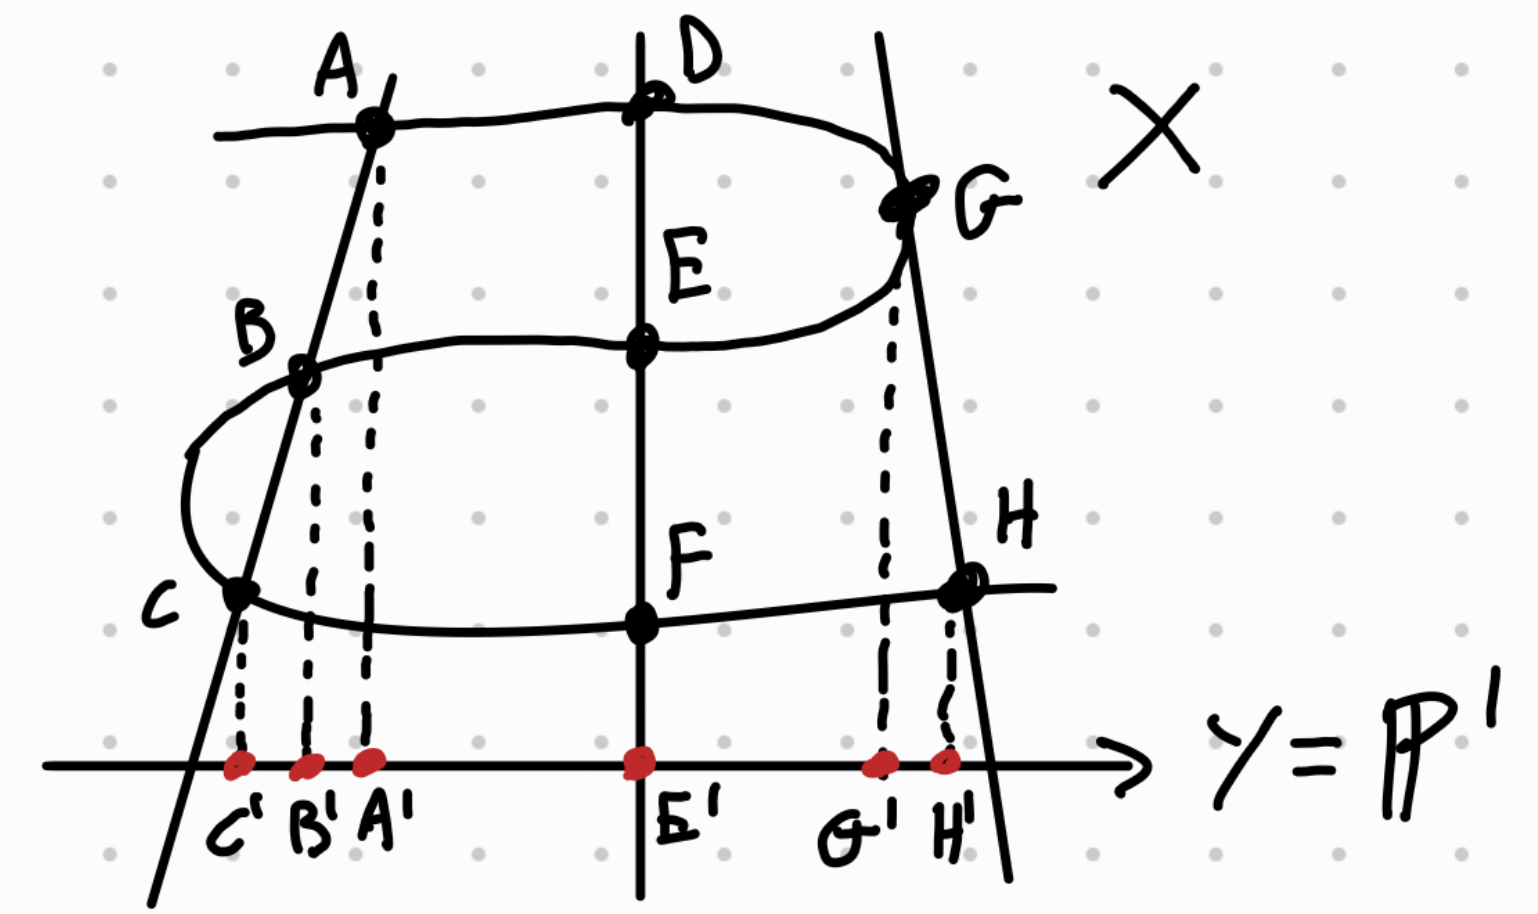
\includegraphics[width=7cm]{Images/degree-pushforward.png}
	\caption{The cycle $A+B+C\sim D+E+F\sim 2G+H$, gets mapped to $A'+B'+C'\sim 3E'\sim 2G'+H'$. In all cases multiplicities are preserved.}
\end{figure}


\begin{proposition}
If $X\to \Spec k$ is proper, then we have a unique map $\deg:CH(X)=CH(pt)\cong \Z$ which preserves dimension (so $[Y]\mapsto 0$ if $\dim Y>0$ and $[pt]\mapsto 1$).
\end{proposition}



\section{Projective space}
Since properness seems to play a big role in this theory, we compute the Chow ring of projective space.

\begin{definition}[]
Let $X\subseteq \Pj^n$ be an irreducible closed subvariety of dimension $k$. The \textbf{degree} of $X$ is the number of intersection points, counted with multiplicities, it has when intersected with $k$ hyperplanes in general position.

Another defition is the following: Let $P(t)=\frac{h(t)}{(1-t)^k}$ be the Poincar\'e-Hilbert series of $X\subseteq \Pj^n$ ($h(t)$ is a polynomial), then the degree of $X$ is $h(1)$.
\end{definition}

\begin{definition}[]
Let $X$ be a scheme of finite type of $k$. We call a finite collection of irreducible locally closed subschemes $X_i$ an \textbf{affine stratification} if 
\begin{itemize}
\item each $X_i$ is isomorphic to some $\A^{k_i}$,
\item $X$ is the disjoint union of the $X_i$,
\item the closure of each $X_i$ us given by a union of some $X_j$.
\end{itemize}
\end{definition}

\begin{theorem}
We have that as graded rings
\[CH(\Pj^n)\cong \frac{\Z[t]}{(t^{n+1})}\]
where $t$ is the class of some linear hyperplane. Moreover, if $X\subseteq \Pj^n$ irreducible of codimension $k$ and degree $d$ then $[X]=dt^k$.
\end{theorem}
\begin{proof}[Sketch]
The proof consists of the following steps
\setlength{\leftmargini}{0cm}
\begin{itemize}
\item Consider the chain of inclusions
\[\cpa{pt}=\Pj^0\subseteq \Pj^1\subseteq\cdots\subseteq \Pj^n\]
given by fixing the last free coordinate to be $0$ to get from one term to the previous one. Consider the differences $U_i=\Pj^i\bs \Pj^{i-1}$, which are all isomorphic to affine space. It turns out that the $U_i$ form an {affine stratification} of $\Pj^n$.
\item Prove that $CH(\Pj^n)$ is generated by the classes of $[\ol{U_i}]$. The idea to prove the result for general affine stratifications. Proceed by induction on the number of strata. Let $U_0$ be a minimal strata and note that beacuse of that $\ol{U_0}=U_0$. By excision we have:
\[\Z=CH({U_0})=CH(\ol{U_0})\to CH(X)\to CH(X\bs \ol{U_0})\to 0\]
and the last bit is a scheme with affine stratification that has one less strata, therefore the Chow ring of the last term is generated by the $[\ol{U_i}]$ for $i\neq 0$ by inductive hypothesis. 
\item Intersecting $k$ hyperplanes gives a $(n-k)$-plane, so $t^k=[(n-k)\text{-plane}]$.
\item Let $M\subseteq \Pj^n$ be an $k$-plane, we have a surjective\footnote{$(n-k)$-plane $\cap$ $k$-plane $=[pt]$, generator of $CH^n(\Pj^n)$} map
% https://q.uiver.app/#q=WzAsMyxbMCwwLCJDSF5rKFxcUGpebikiXSxbMSwwLCJDSF5uKFxcUGpebikiXSxbMiwwLCJDSChwdCkiXSxbMCwxLCJcXGNkb3QgW01dIl0sWzEsMiwiPSIsMyx7InN0eWxlIjp7ImJvZHkiOnsibmFtZSI6Im5vbmUifSwiaGVhZCI6eyJuYW1lIjoibm9uZSJ9fX1dLFswLDIsIlxcZGVnIiwyLHsiY3VydmUiOjJ9XV0=
\[\begin{tikzcd}
	{CH^k(\Pj^n)} & {CH^n(\Pj^n)} & {CH(pt)}
	\arrow["{\cdot [M]}", from=1-1, to=1-2]
	\arrow["\deg"', curve={height=12pt}, from=1-1, to=1-3]
	\arrow["{=}"{marking, allow upside down}, draw=none, from=1-2, to=1-3]
\end{tikzcd}\]
and the full composition is the degree map, so this is also injective ($[X]$ is in the kernel when it has empty intersection with general $M$ and this cannot happen if $X$ has codimension $k$).
Thus $CH^k(\Pj^n)\cong \Z$ and this map is actually an isomorphism of abelian groups. Moreover, if $[X]\in CH^k(\Pj^n)$ then\footnote{by definition, the degree of an $(n-k)$-subvariety is the number of intersections with a general $k$-plane} 
\[[X][M]=\deg X [pt]=\deg X t^n=(\deg X t^{k})t^{n-k}=(\deg X t^{k})[M]\] 
and so $[X]=\deg Xt^k$.
\end{itemize}
\setlength{\leftmargini}{0.5cm}
\end{proof}

To get some practice with this ring we conclude with the following exercise

\begin{exercise}
In $\A^2$ draw three circles $C_1,\ C_2,\ C_3$. 
\begin{figure}[!htb]
	\centering
	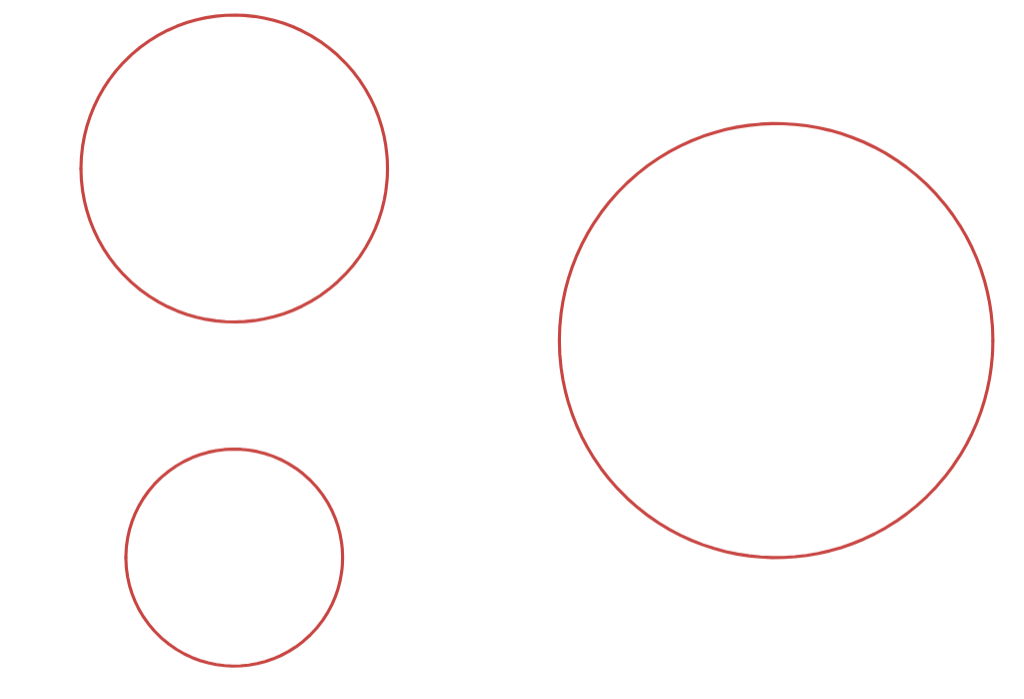
\includegraphics[width=5cm]{Images/Three-circles.png}
\end{figure}

How many circles can be drawn which are tangent to $C_1$, $C_2$ and $C_3$?
\end{exercise}
\begin{proof}[Solution]
A circle in the plane is given by an equation of the form $(x-A)^2+(y-B)^2=C$. If we homogenize we see that the two points at infinity $[1:\pm i:0]$ always lie on such a homogenized circle. We may therefore define a circle in $\Pj^2$ to be a conic which passes through these two points.

Recall that conics in $\Pj^2$ are parametrized by $\Pj^5$ by looking at the coefficients in their general equation
\[ax^2+bxy+cy^2+dxz+ezy+fz^2=0.\]
By imposing the fact that the circles should go through two distinct points we get that circles are parametrized by a $\Pj^3$. More precisely, they correspond to the intersection of the two hypersurfaces $a+bi-c=0$ and $a-bi-c=0$ in $\Pj^5$.


What does it mean for a circle to be tangent to another fixed circle $C$? Let $Z_C=\cpa{\text{circles tangent to $C$}}\subseteq\Pj^3$ and consider the pairs
\[\Phi=\cpa{(r,D)\mid r\in C,\ D \text{ circle tangent to $C$ at $r$}}.\]
We have two projections $\Phi\to C$ and $\Phi\to Z_C$. Note that the fibers of $\Phi\to C$ are isomorphic to $\Pj^1$: up to translation, suppose that $r=0$. If $D$ is some circle which is tangent to $C$ at $0$ then all circles which are tangent to $C$ at that same point are re-scaled versions of $D$. 

\begin{figure}[!htb]
	\centering
	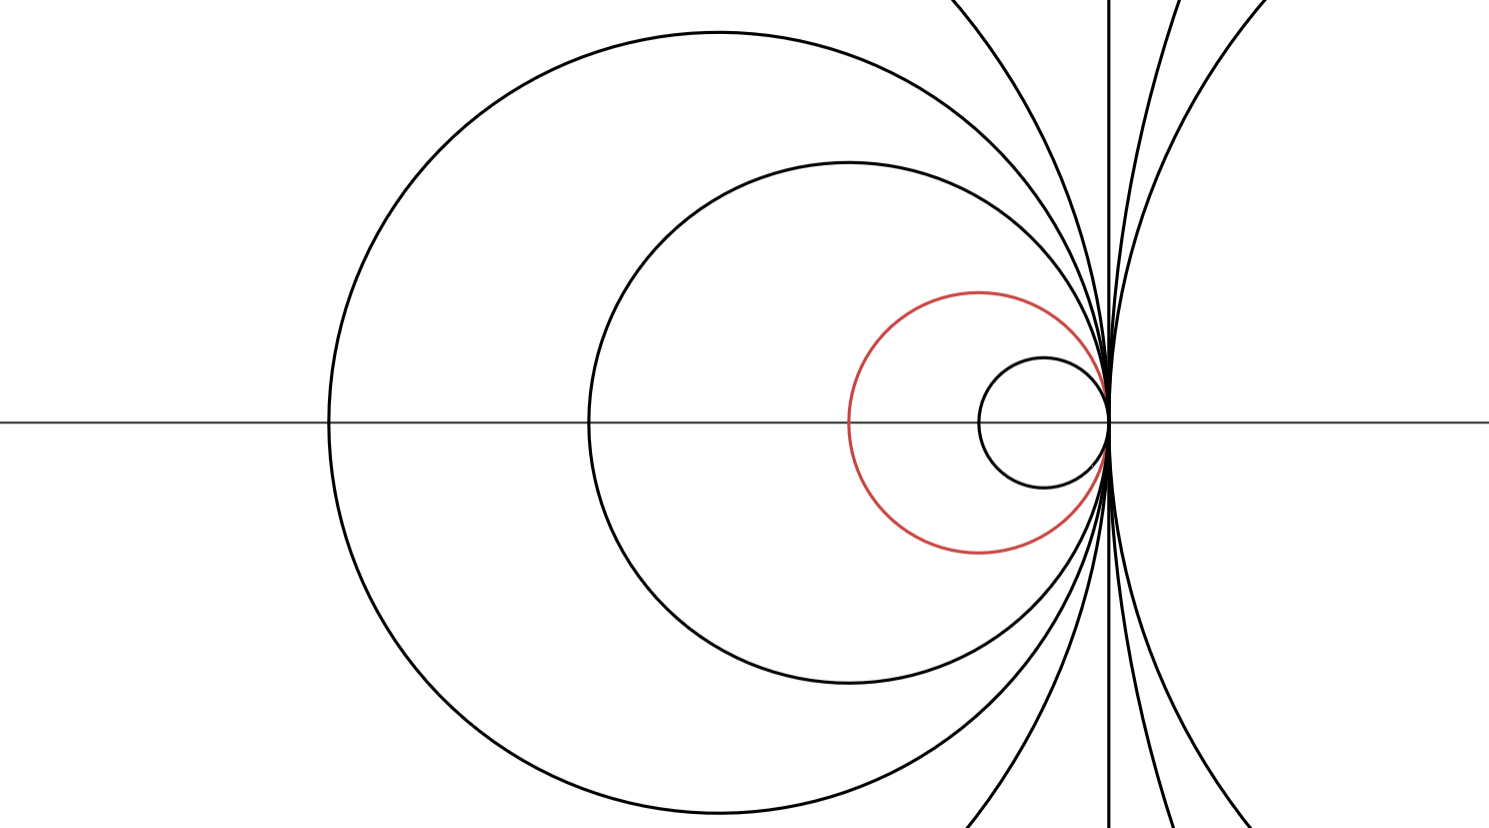
\includegraphics[width=7cm]{Images/pencil-of-tangent-circles.png}
\end{figure}

So $\Phi$ should be a surface of some kind (fiber bundle over a circle with fibers given by $\Pj^1$). This surface should have degree 2 because tangency between a circle $D:(x-a)^2+(y-b)^2=c$ and a fixed circle $C:(x-a_0)^2+(y-b_0)^2=c_0$ is checked by imposing that the following system of equations has a double solution 
\[\begin{cases}
	(x-a)^2+(y-b)^2=c\\
	(x-a_0)^2+(y-b_0)^2=c_0
\end{cases}\]
and the way we impose that is by setting the discriminant of a resulting quadratic equation to be 0. The fact that the degree should be two comes from the fact that the discriminant has degree two in the coefficients of the equation.

Moreover, $Z_C$ is birational to $\Phi$ (from a circle in $Z_C$ we can get the point of tangency it has with $C$).

So $Z_{C_1}\subseteq\Pj^3$ is a surface of degree 2. In the Chow group $CH(\Pj^3)$ we thus have $2t=[Z_{C_1}]$ and so
\[[Z_{C_1}\cap Z_{C_2}\cap Z_{C_3}]=[Z_{C_1}][Z_{C_2}][Z_{C_3}]=(2t)^3=8t^3\]
and $8t^3\in CH(\Pj^3)$ is the class of eight points.

\begin{center}
	\textit{The number of tangent circles we were looking for is therefore $8$ when the three circles are in sufficiently general position.}
\end{center}
\end{proof}
















